\documentclass{article}
\usepackage{graphicx}
\usepackage[utf8]{inputenc}
\usepackage{amsmath}

\begin{document}

    \section*{Chosen manipulator}

    For this task I decided to chose an anthropomotphic manipulator with yzy spherical wrist.

    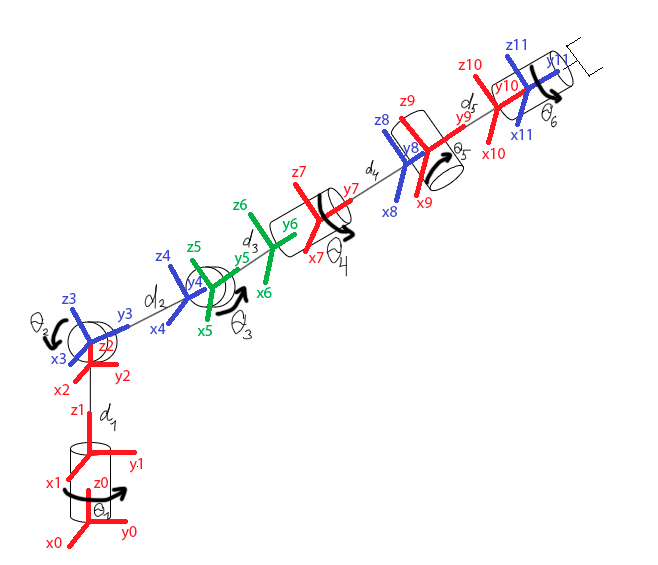
\includegraphics[width=\linewidth]{manipulator_scheme}

    \section*{Forward kinematics}

    I found position of the end effector in this way:

    $$P_{end} = P_{base} R_z(\theta_1) T_z(d_1) R_x(\theta_2) T_y(d_2) R_x(\theta_3) T_y(d_3) R_y(\theta_4) T_y(d_4) R_z(\theta_5) T_y(d_5) R_y(\theta_6)$$

    where $P_{base}$ is an identity 4x4 matrix, $R_{axis}(\theta)$ is a rotation matrix in homogeneous representation on given angle $\theta$ around given axis and $T_{axis}(d)$ is a translation matrix in homogeneous representation on given axis on given distance.

    Plots obtained:

    \begin{figure}[h]
        \centering
        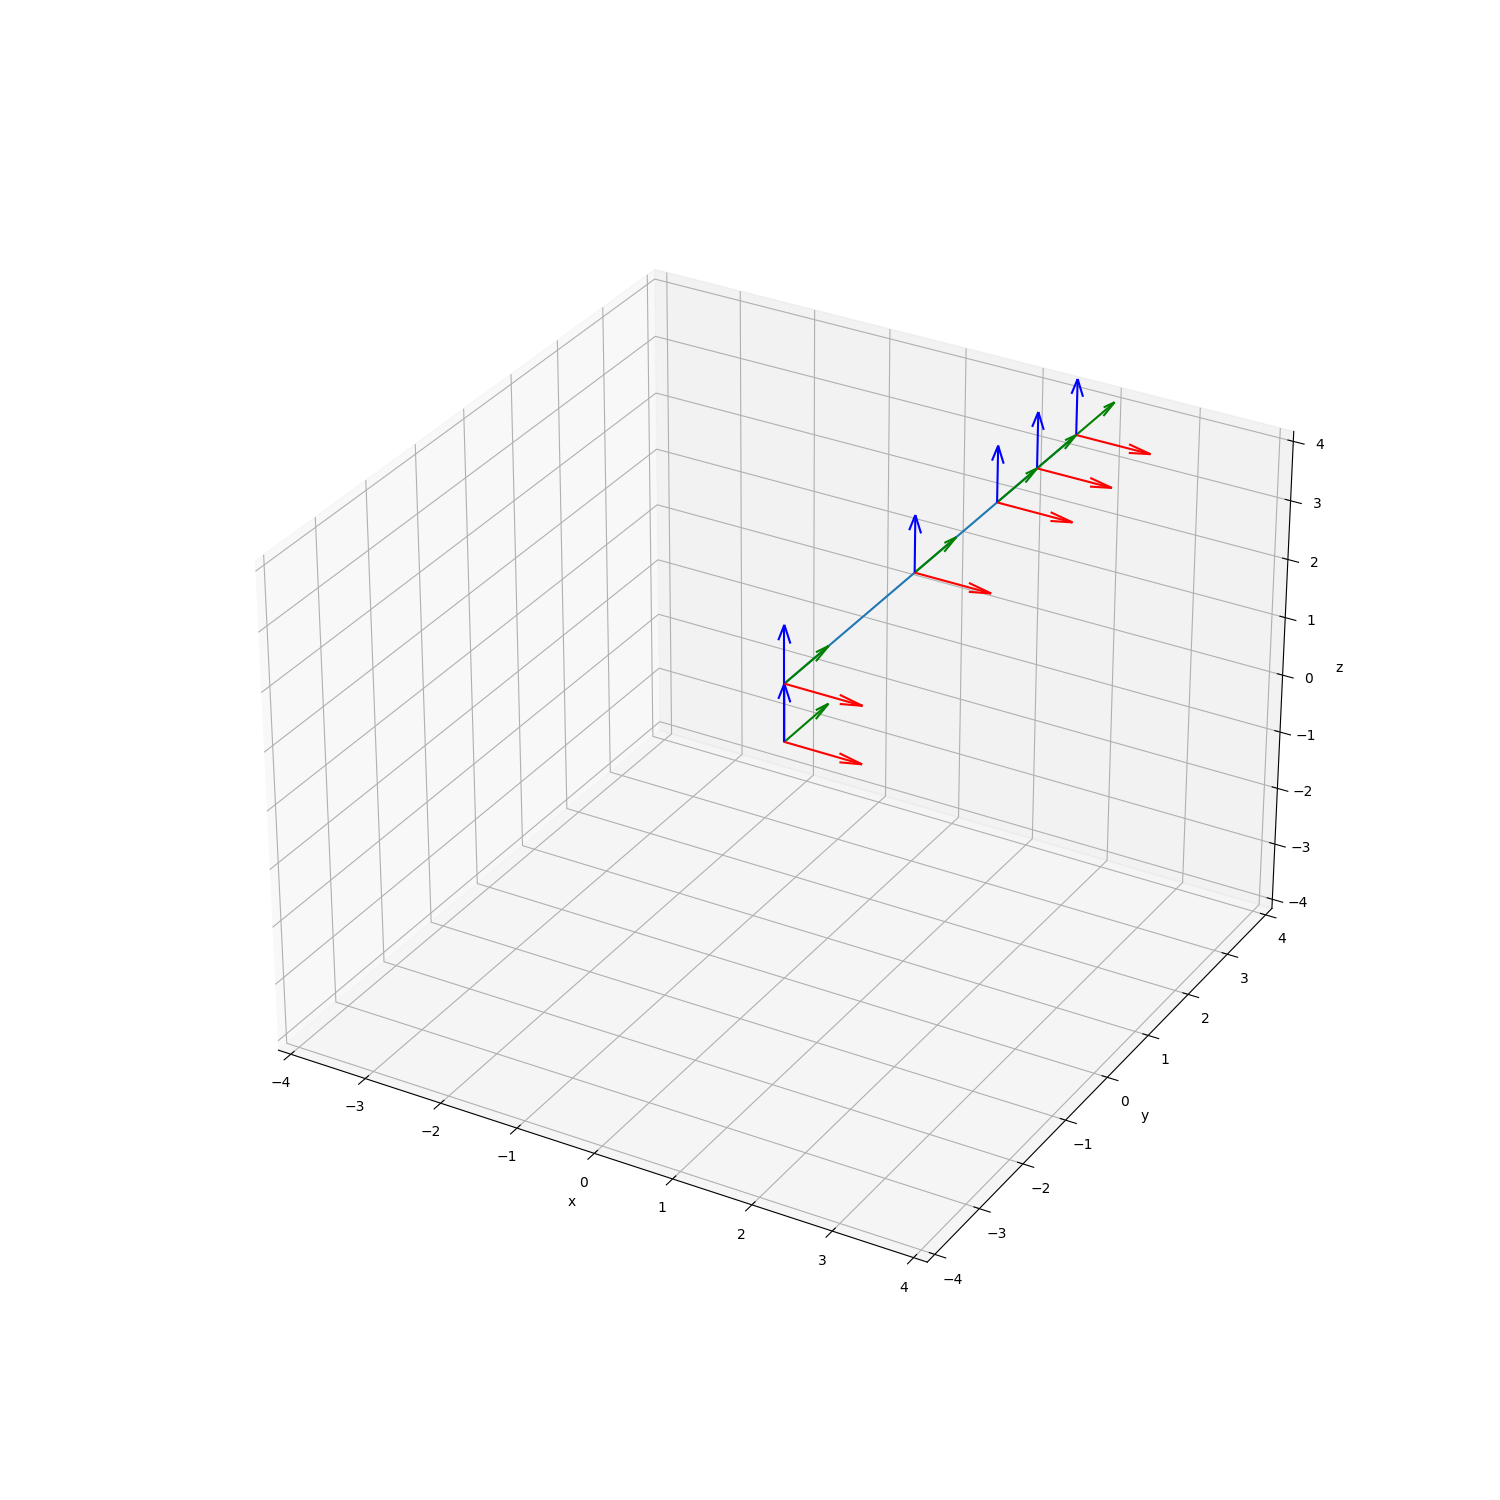
\includegraphics[width=\linewidth]{forward_zeros}
        \caption{Obtained positions for zero angles}
        \label{fig:figure1}
    \end{figure}
    
    \begin{figure}[h]
        \centering
        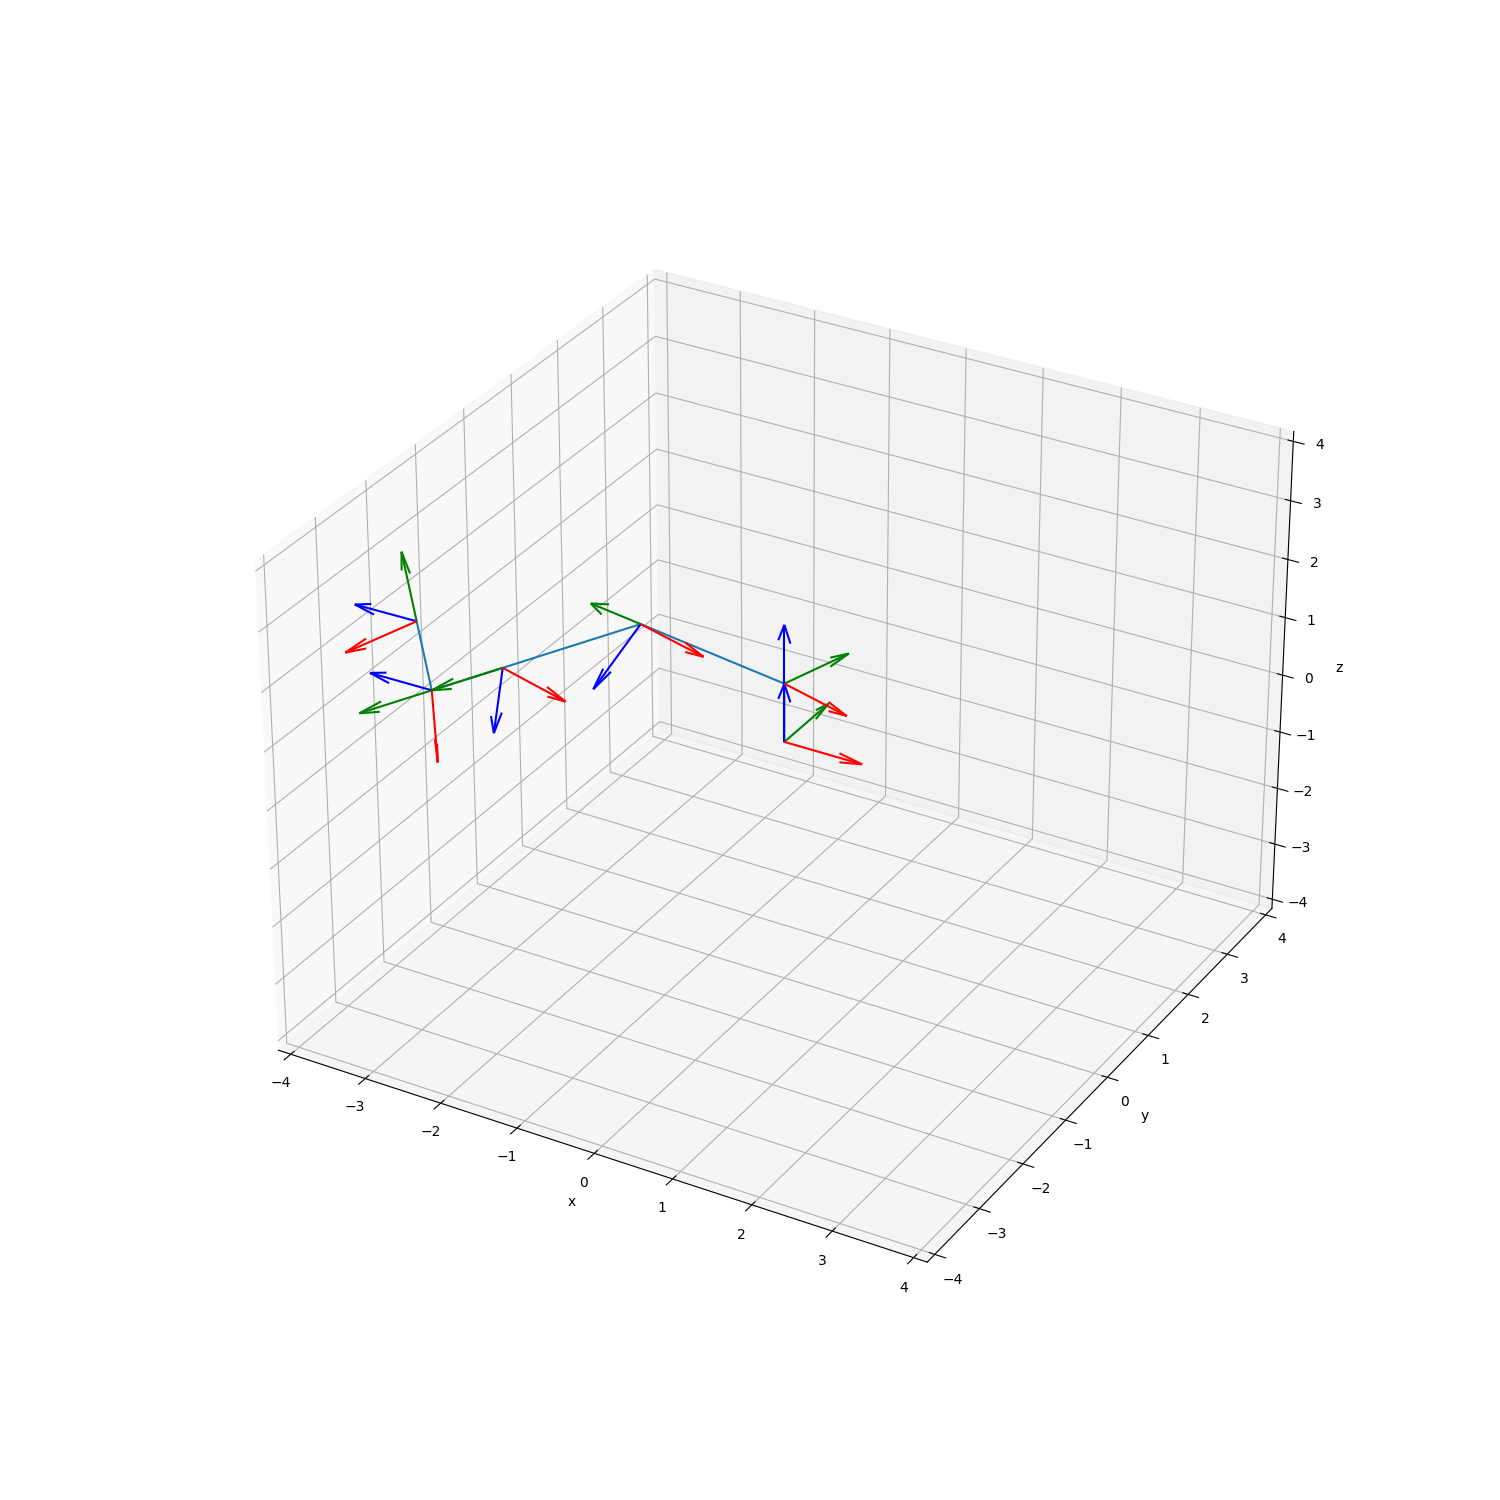
\includegraphics[width=\linewidth]{forward_random}
        \caption{Obtained positions for random angles}
        \label{fig:figure2}
    \end{figure}
    
\end{document}